\documentclass{article}
\usepackage{csvsimple}
\usepackage{amsmath}
\usepackage{amssymb}
\usepackage{graphicx}
\usepackage{hyperref}
\usepackage{wrapfig}

\begin{document}

%insert your content here..

\section{Student content}


%\maketitle
\begin{figure}[h!]
\centering

\includegraphics[width=.5\columnwidth]{picture-nazmus.jpg}
\caption{Picture of Nazmus.}
\label{fig:my-picture}
\end{figure}

\section{Introduction}

Hello. This is my immense pleasure to introduce myself here. My name is Nazmus Sakib, and I am from Bangladesh. I am a first-year Ph.D. student studying in the Cybersecurity program at the Computer Science Department at the University of Colorado Colorado Springs. I obtained a research-based Master of Computer Science degree from the University of Malaya, Malaysia in 2020. Prior to that, in 2012, I graduated with a B.Sc. (Engineering) in Computer Science and Engineering degree from the Shahjalal University of Science and Technology, Bangladesh. Currently, I am working as a Graduate Research Assistant (GRA) at the Networked System Security Lab at UCCS under Dr. Sang-Yoon Chang's supervision. I am interested in working in diverse computer science research fields including Blockchain, Bitcoin, Anomaly Detection, and Machine Learning.

\section{Related code}

I have been working on a research project titled ``Bitcoin Network Performance Analysis Using Annonymous Routing''. Here, we have logged Bitcoin Peer-to-Peer network and collect networking data.
Check the git repo here: https://github.com/peer-connectivity-estimator/bitcoin-network-logger

\section{Ask question here}

\subsection{Carlos: What do you think is the future for blockchain and bitcoin? And the other applications that it can have in the future?}

\subsection{Alharbi: How can user privacy concerns be addressed when using Bitcoin?}
%\documentclass[article]{IEEEtran}
%\usepackage[utf8]{inputenc}
%\usepackage{graphicx}
%\usepackage{cite}
%\usepackage{url}

\title{Week 4. GitHub Assignment \\
\large UCCS CS 6000 Computer Science Research}
\author{Jose Luis Castanon Remy}
\date{September 2022}

%\begin{document}

\maketitle

\section{Myself}

During my experience working as a cybersecurity analyst, I have always faced different issues related to the field. I always thought no one had the interest to solve or even address these issues. Common issues that I have found while working are disinformation, disinterest, and uncontrol. This constitutes my second goal. I would love to research and solve issues within the cybersecurity field that no one is paying attention to. One of these issues is the fact that many companies that I had the opportunity to work for, all lack a proper inventory of software leading to security issues.



In addition to my goals and expectations, I consider myself to be very creative. I love to paint. I consider myself an artist in multiple disciplines. I love charcoals and pencils. I am currently learning color theory and how to paint figurines and build dioramas. Apart from my artistic face, I love biking. It is the best way for me to add cardio to my gym routine without getting bored.

I will be completing my Ph.D. in Cybersecurity.


\begin{figure}[htp]
    \centering
    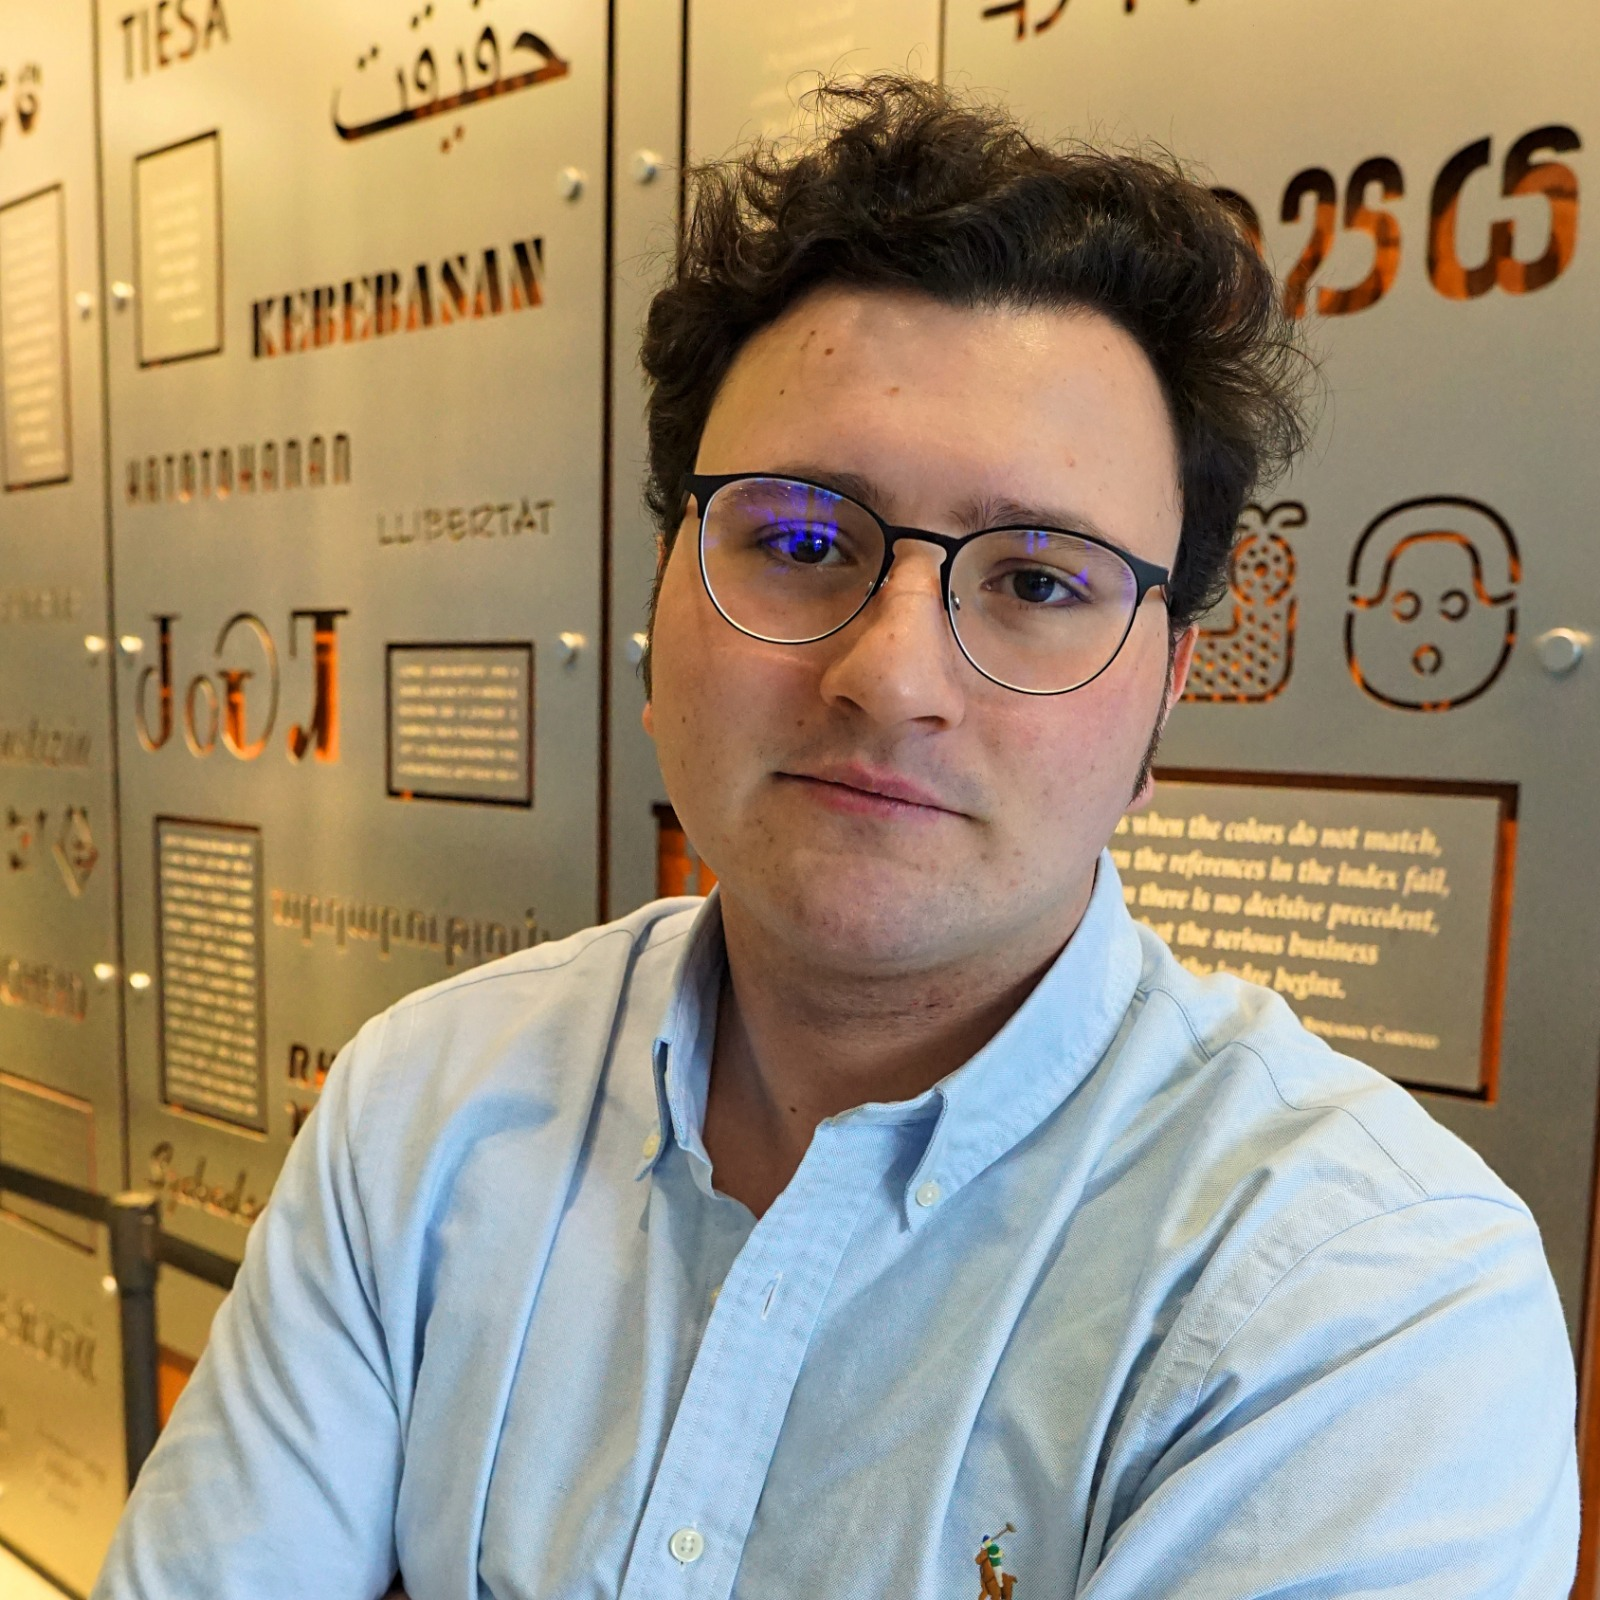
\includegraphics[width=4cm]{UCCSProfileIMG.jpg}
    \caption{An image of myself}
    \label{fig:myself}
\end{figure}


\section{Git Code}
I am currently working on a research related to security and software maintenance. It is a broad topic but I will be trying to narrow it down as I advance with my story.

Maintenance is a large part of every security team. Maintenance represented more than 50\% of the tasks and duties within the last security team I worked with. Part of the maintenance process was related to cleaning. There is a broadly known app related to cleaning called CCleaner. Cleaning helps solve issues directly linked to unused files within installation folders, cache folders, etc. CCleaner helps detect and clean up these files.

Currently, the tasks that CCleaner can perform are limited. For this reason, I have chosen the following Git repo, Winapp2, \url{https://github.com/MoscaDotTo/Winapp2}.

Winapp2 extends the cleaning routines of CCleaner. Winapp2 compiles a list of keys, as a configuration file, for CCleaner to check more applications to clean.
This is highly related to my research as I would like to build something that can map the stack of software within a computer system.
Winapp2 is not also compatible with CCleaner but with other cleaning apps like BleachBit, System Ninja, Avira System Speedup, Tron, and R-Wipe \& Clean. Winapp2 repository contains Winapp2ool, which helps maintain, manage, download and deploy Winapp2, \url{https://github.com/MoscaDotTo/Winapp2/tree/master/winapp2ool}


\section{Questions}
Please, leave your questions after this line.

You say your topic is broad so what types of softwares have you narrowed down so far? Or if you havent done anything yet to narrow that part down then have you looked at maybe different types of attacks to investigate, like maybe what is the most prominent attack among software vs effectiveness of these attacks? -Noah Rodgers
My topic is not focused specifically on finding vulnerabilities. It is more focus on the discovery part of the software itslef. This "discovery" is what I call mapping. Having a map of the software implies a better future protection.

JTs question/comments:  I think it's cool that you are looking at security from the maintenance perspective.  Was there ever a time that you were able to use this approach with success as an analyst?  What companies or organizations have you provided services for?
Yes, working as a security analyst is highly related to the maintenance perspective. You need to give guidence in most of the processes related to the security of the company. I am not allowed to speak about my clients, sorry.

\KoraComments{Do you have an example of what a map might look like?}
I do not but I think of the map as heat map or a bubble graph like map.

\bibliographystyle{IEEEtran}
\bibliography{refs}

%\end{document}

%\documentclass[article]{IEEEtran}
%\usepackage[utf8]{inputenc}
%\usepackage{graphicx}
%\usepackage{cite}
%\usepackage{url}

\title{GitHub Assignment}
\author{Noah Rodgers}
\date{September 2022}

%\begin{document}

\maketitle

\section{About Me}

Hello, my name is Noah Rodgers I am a Graduate Student in the Master of Cyber Security program at UCCS. I work at the Aerospace Corporation as an intern Cyber Specialist working with NASA and the Space Force. What I hope to gain from this course is how to properly conduct my research. As well as write my papers with the correct language and grammar. I hope this will further my research work as I start my work for Dr. Chang. I am working on disrupting satellite communications using different methods examining viability, and effectiveness. I am also hoping that this course will touch on how to write and prepare my thesis for my master’s program. Something personal about me is that I love to go sand boarding at the Great Sand dunes. I also like to long board to class from my home on sunny days although I’m not that good at it but I haven’t crashed yet, so I guess that’s a plus. I got my Bachelors in Game design and Development at UCCS and got my minor in computer science so I’ve been working on filling in the gaps for cyber security. I look forward to what this class has to offer.



\begin{figure}[!htb]
    \centering
    
\includegraphics[width=85mm, angle=90]{Me1.jpg}
    \caption{\textbf{Picture of Myself}}
    \label{fig:jamequation}
\end{figure}


\section{Git Code}
A collection of Resources for budding SAT hackers (Satellites, not the test¯\_(ツ)_/¯).

This is the basic hack a sat github repo where you can learn and train to help better security for these devices.

https://github.com/deptofdefense/hack-a-sat-library

\section{2 Questions to answer}
How different is the attack vector when facing a hacking process aiming for satellites? - Jose Remy



\bibliographystyle{IEEEtran}
\bibliography{refs}

%\end{document}



\title{Lattice based cryptography}
\author{Qaiser khan }
\date{August 2022}


\maketitle

\section{About Me}
 This is Qaiser khan from Pakistan. Pakistan is geographically located in South Asia. I am a PhD student at UCCS, Doing PhD in security and works with Dr Sang Yoon Chang at Network Security and System lab.  I have completed my master’s in information security (with a major in Cryptography) from one of the prestigious universities of Pakistan i.e. National University of Science and Technology, Pakistan. Then I got Research Assistant-ship at UCCS.I like travelling, hiking and love to play with mathematical stuff.I am taking this course CS-6000 because my advisor and my lab mates suggested to take this course and this will help in your research and can learn more new stuff and tools like Zotero, overleaf and also how to use google scholar to find your interest paper more quick.This subject will help to know about good conference, journals and impact factors of journals. My research interest in post quantum cryptography as we know that after Quantum computer came there will be security threat to recent asymmetric algorithm like RSA, Diffie-hellman and all algorithm that is based on factorization and discrete logarithms \cite{alagic2019status}. So to secure the confidential data NIST (National institute of standards and Technology) in 2016 announced for post quantum algorithms that should be quantum resistance\cite{raavi2021security}.

\begin{figure}[htp]
    \centering
    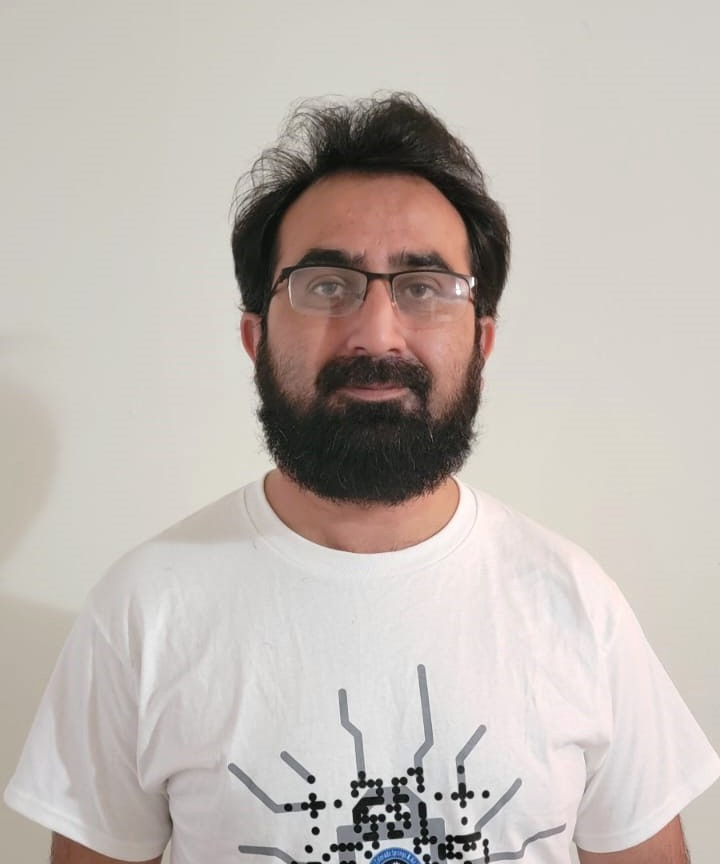
\includegraphics[width=6cm]{qaiser.jpeg}
    \caption{Qaiser khan}
    \label{fig:Qaiser}
\end{figure}

\section{Git Code}
I am working on post-quantum cryptography, so here is the link to a popular library that contains all the NIST standardization source code files for the post-quantum algorithms:
\href{https://github.com/open-quantum-safe/liboqs}{https://github.com/open-quantum-safe/liboqs}.

\section{Any Questions?}


Hi Qaiser, trust you are well.
Your research area seems interesting, does asymmetric algorithm give promise to unbreakable security?...This is Rono
%

% What are the likely methods used to secure asymmetric algorithms?
Do you plan on creating or revising any of the post quantum algorithms? Also, which one do you think shows the most promise/strength? - Dustin Trujillo 

%
%

\section{Ken Lee}
\subsection{intro}
I am a first year PhD student under Dr. Brown.  
We have discussed several ideas, and I have a list of conferences and journals that he publishes to most often for reference.
I am really enjoying the material in this class, though I really have to change habits so that I can spend blocks of time reading papers that I may eventually use.  
Even more import to me, is the information that I gain from the papers to stay current in my field.
Besides school and working fulltime, I enjoy sailing as my hobby to really unwind.  
Below is a picture of me at the helm of our 19 ft Flying Scot sailboat named Fin and Tonic.
\begin{figure}[!htb]
\centering

\includegraphics[width=0.5\textwidth]{sailing_flyingscot.jpg}
\end{figure}

\subsection{git repo}
\url{https://github.com/kalee/Schelling-Segregation.git} This is a project that I worked on in another class.  
It is Java code that runs the Shelling Segregation model.  
This is related to my field of research in that it is using agents that work locally towards a specific goal.  
A goal that wasn't worked on was worst-case analysis.  
We setup a boundary of a maximum of 100x100 grid squares.  
Much larger, and it really takes a long time to complete.  
There is a lot of code to run
through, and determining $\Theta$ for worst case was not the point, though could be included.

\subsection{Questions}
\textbf{Question 1:} Hey Ken! How did you decide to study at UCCS?\\
I have a son who is graduating from UCCS this December with a BS with I believe is a triple major (EE, Mathematics, and Computer Science).  I'm obviously pretty proud of his accomplishments.  Well, a few years ago, I was taking C Programming at ACC.  I was not really happy with what I got out of it.  I did really like the price, but it just wasn't worth it to me.  I talked to my son, and he mentioned some of the classes in CS and a some of the work he was doing.  I was sold at that point.  I started with 1450, then jumped up to 5720.  I talked to my professor about what I wanted to accomplish, which is really solving problems, and discussed the PhD program and how that would help me to attain my goals.  That is the short version, but is how I decided to study at UCCS.\\


%% This is a skeleton file to create IEEE style Bibliography list. There is a guide added "create-manual-bib-entry.txt" to manually create popular types of references such as PhD thesis, website, unpublished work etc.
%%
%% Modified by K. Reaz( kahn.reaz@ieee.org)
%% Support sites:
%% http://www.ieee.org/

%%***********************************************************
%% Legal Notice:
%% This code is offered as-is without any warranty either expressed or implied; without even the implied warranty of MERCHANTABILITY or FITNESS FOR A PARTICULAR PURPOSE! 
%% User assumes all risk and can modify as s/he wants.

%%***********************************************************

%package list
\documentclass[conference]{IEEEtran}
\usepackage{cite}
\usepackage{cite}
\usepackage{amsmath,amssymb,amsfonts}
\usepackage{algorithmic}
\usepackage{graphicx}
\usepackage{textcomp}
\usepackage{xcolor}
\usepackage{dirtytalk}
\usepackage{csquotes}
\usepackage[export]{adjustbox}
\usepackage[pdftex]{graphicx}

\def\BibTeX{{\rm B\kern-.05em{\sc i\kern-.025em b}\kern-.08em
    T\kern-.1667em\lower.7ex\hbox{E}\kern-.125emX}}
\author{Ali Al Shami$^{1}$}

\thanks{Ali Al Shami with the Computer Science Department, University of Colorado Colorado Springs, Colorado Springs, CO, 80918 USA e-mail:(aalshami@uccs.edu)}
\begin{document}
%Here goes the title
\title{Journal 1}
\maketitle

%Main body starts
\section{Introduction}
I am Ali Alshami, a Ph.D. student in computer science and a Graduate Research Assistant (GRA) at the Vision Security Technology (VAST) Lab, the University of Colorado Colorado Springs (UCCS).

My goal for the course is to finish and submit a survey paper on human action recognition and prediction and start a new paper that focuses on predicting the future movement of humans based on human pose estimation and motion information. The survey paper reviews and evaluates the recent human actions recognition and prediction papers based on vision and machine learning. The new work will be focused on predicting the future movement of humans in video based on past movement, motion information, and human pose estimation.

I hope to learn more about improving my research skills and what I must consider becoming a better researcher. I am also curious about how to convert research that we are working on to a product you and what things we need to consider to make it a successful product.

I enjoy outdoor activities, including running, hiking, mountain biking, tennis, pickle-ball, and snowboarding. I also like reading and playing piano sometimes.
\begin{figure}[hbt!]
    \centering
    
\includegraphics[width=5cm]{alshami.jpg}
    \caption{ }
    \label{fig:Remove}
\end{figure}
\section{Ask question here}
If you dont mind me asking what was your masters and bachelors in because Im curious on what led to that specific topic of research? If its the same as your Ph.D. then what did lead to you becoming intrested in your area of research? -Noah Rodgers

\bibliographystyle{IEEEtran}
\bibliography{main}

\end{document}

% \documentclass{article}
% \usepackage[utf8]{inputenc}
% \usepackage{graphicx}
\graphicspath{ {./images/} }
%\usepackage{hyperref}

\title{Turner  CS600}
\author{James Turner}
\date{September 2022}

%\begin{document}

\maketitle
\newpage
\section{Old Stuff from Assignment 1}
My name is James Turner and I am an active-duty Army Chief Warrant Officer 3 (CW3).  I have served a total of 17 years with 12 years as a Cyber Electromagnetic Warfare (EW) Technician.  This job field is extremely challenging because the technology in the marketplace and capabilities used by our adversaries is constantly changing.  However, it also stimulates innovation and creative thinking and is rewarding when you are part of a team that finds solutions to complex problems.

Recently, I was accepted into the Army’s Advanced Civil School (ACS) program that allows me to attend school full-time and complete a Master’s degree while on active duty.  I have been accepted at UCCS in the Cybersecurity Master of Engineering program, and I am a first term student.  I chose to study cybersecurity because my job field is closely connected with wireless applications and wireless security, and I realized that there is significant job growth in the cybersecurity field.

One of the primary outcomes that I desire from the CS6000 course is to become a more proficient writer and researcher.   I already possess some research and writing skills through my professional military education and on the job experience.  However, military style of writing differs from academia in that the military focuses on a “bottom line up front” perspective and tends to leave details out of formal documents.  I also hope to achieve a greater array of methods that help me conduct more thorough and rigorous research.

Another goal I desire from this course is to enhance my critical thinking.  The military embraces and teaches critical thinking at all levels of leadership education, but I want to gain a greater ability to analyze and test information with scientific methods.  The preponderance of my degree plan and research will be analyzing other tests and scientific data, so I want to be prepared to understand and evaluate those results.  I will need to sharpen my ability to challenge assumptions of others, including myself so that I can become a better researcher.

\begin{figure}
    \centering
    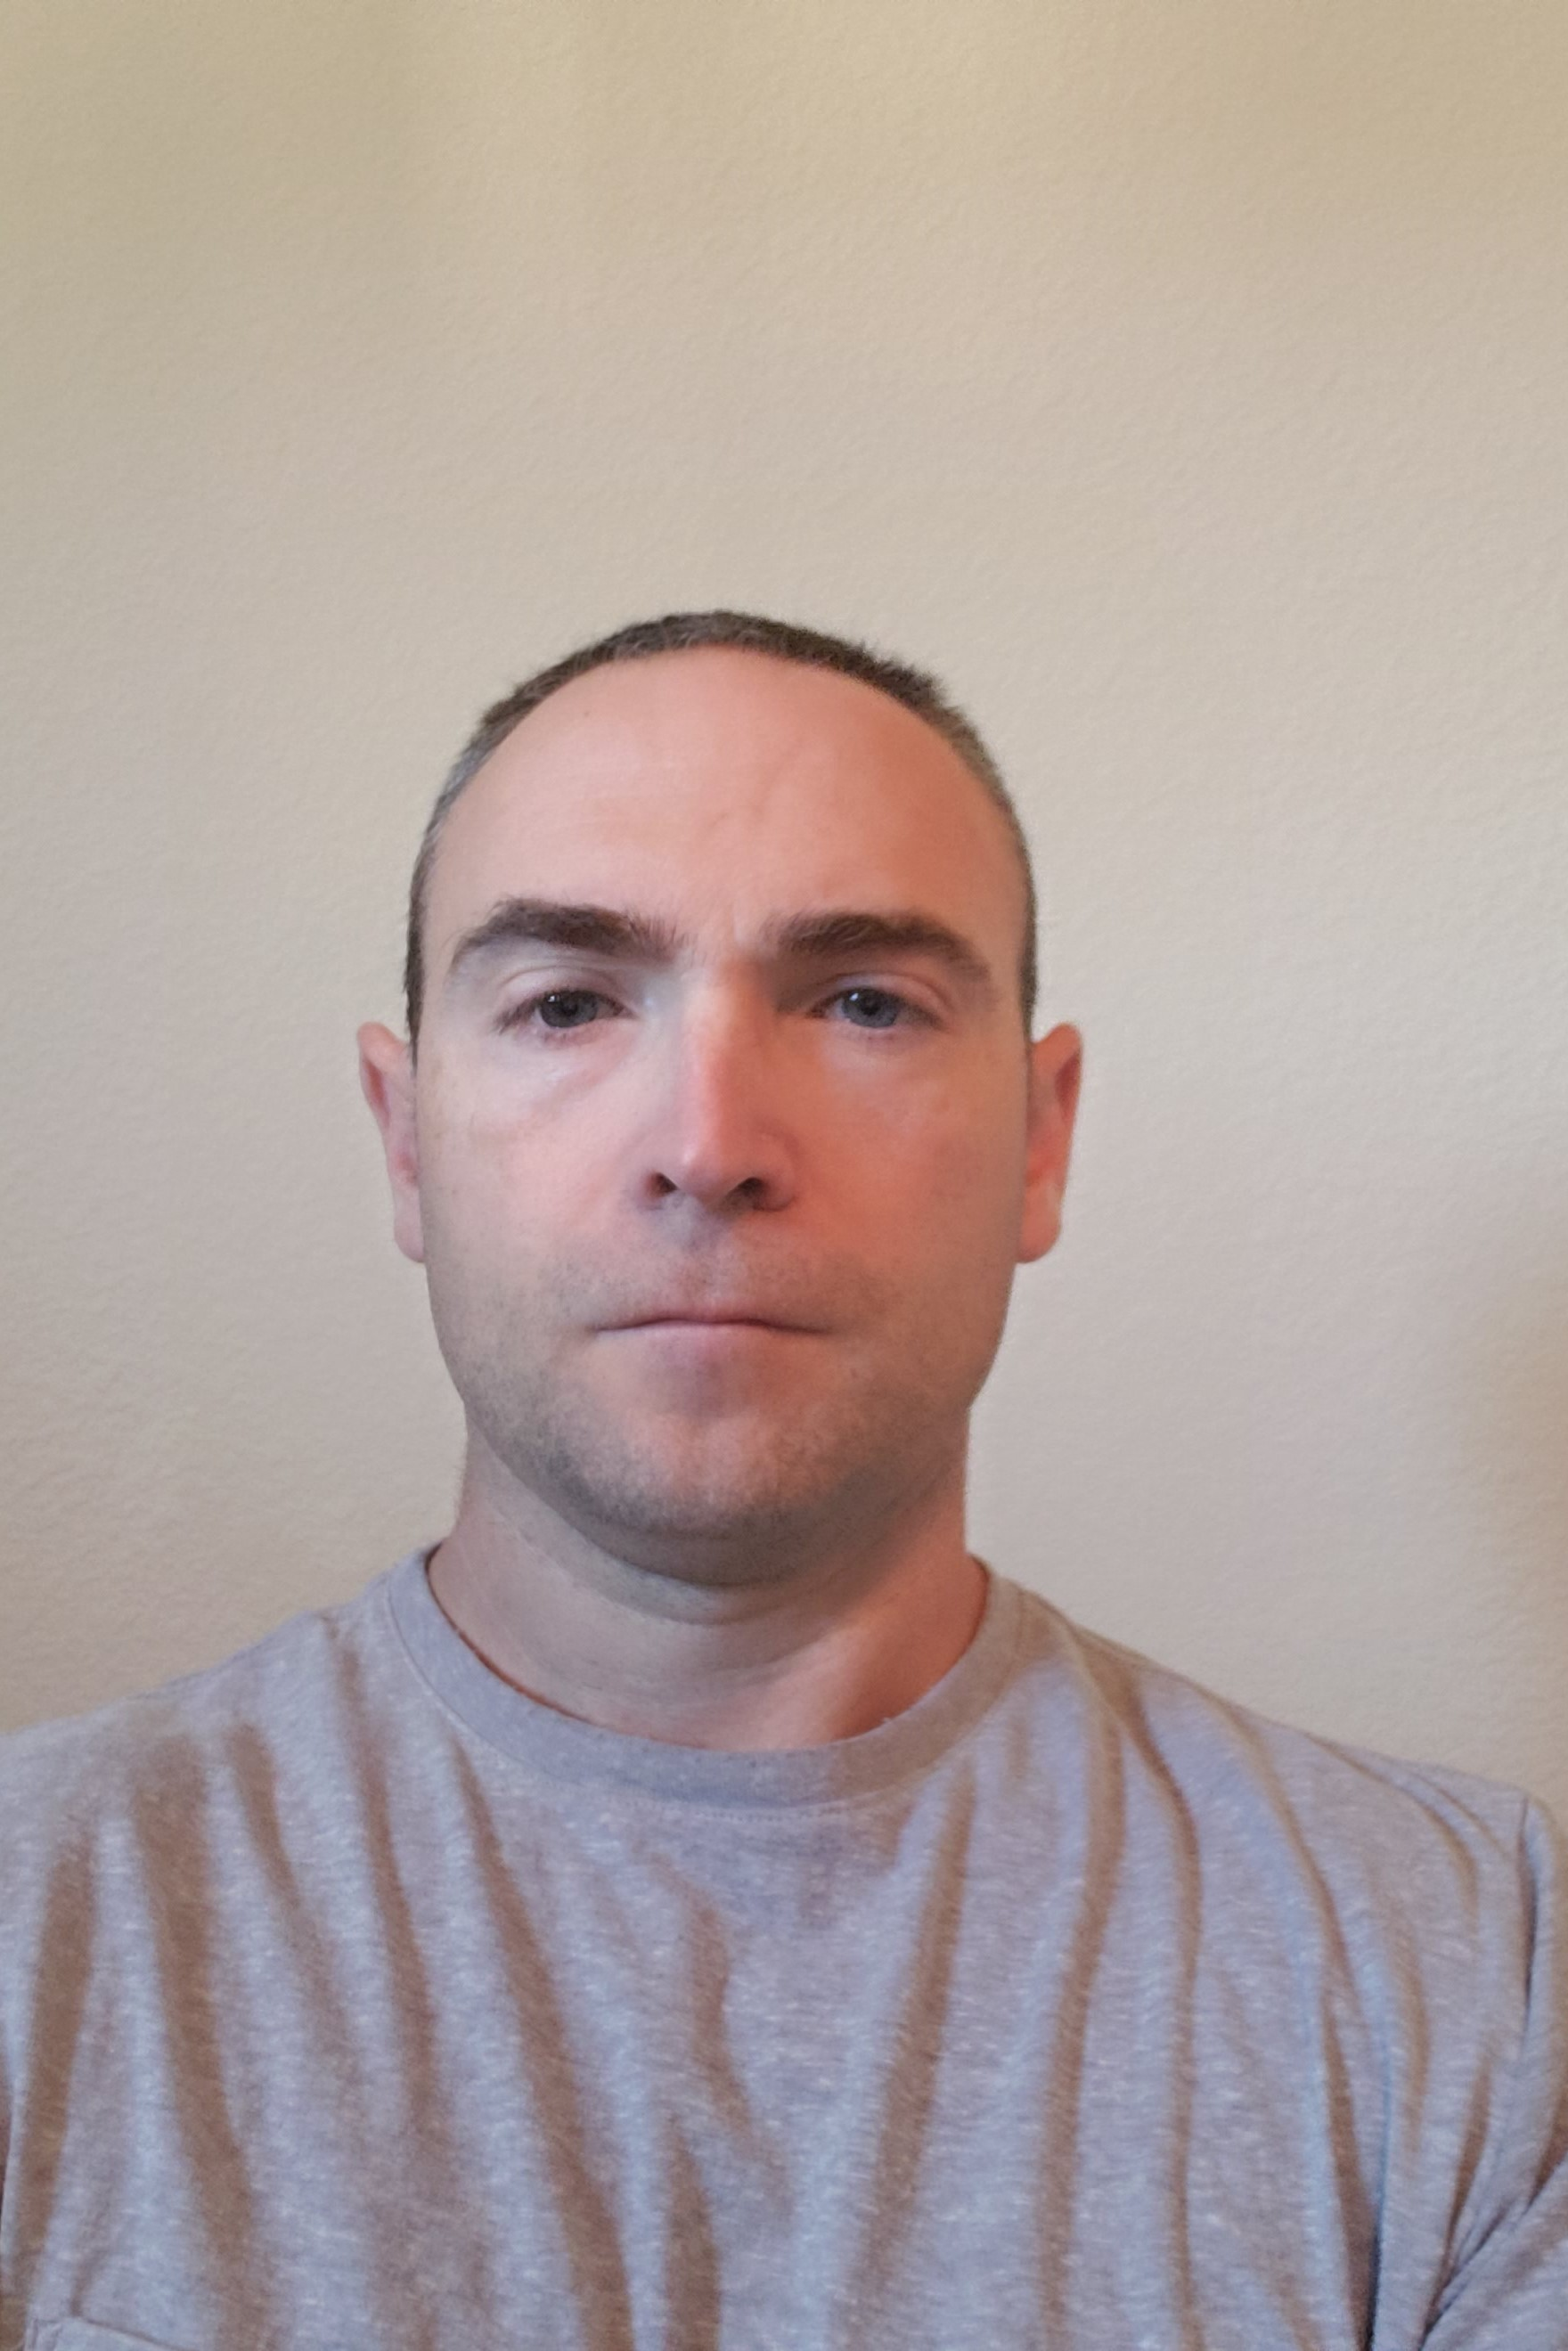
\includegraphics[scale=.1]{self pic2.jpg}
    \caption{me}
    \label{fig:me}
\end{figure}
%\newpage
\section{Github Code on Cognitive Radio}
This repository in Github contains a novel algorithm that uses linear processing to characterize the radio frequency environment in order to enable secondary users' ability to use unoccupied electromagnetic spectrum space.  The link is provided below.
\url{https://github.com/parthgargava/Cognitive-Radio-Networks}

\section{Questions}
What is the main topic that you like to work on for your master thesis, and how do you think that can benefit that army? Ali AlShami
\newline
\paragraph{}
Answer: If I still go the Thesis track then I will discuss some form of wireless security from an avaiability (redundancy and resiliency) and confidentiality perspective.  I still don't know what wireless application I will choose from.  I might focus on 5G or some new type of technology such as reconfigurable intelligent surfaces. 
\paragraph{}
Are you hoping to work on a theoretical or hands-on approach to electronic warfare? I imagine you get a fair share on hands-on experience already. -Katrina
Answer: If I can do live expirementation then that's what I will do.  Yes, I do have plenty of hands-on experiences with different forms of radios and their applications.  However, I need to get stronger from a theoretical standpoint as well.  When you play around with equipment, sometimes it's easy to lose track of the fundamentals in the design of that same equipment.

Nazmus: Have you used PKI in your research?

%\end{document}

\documentclass{article}

\usepackage[english]{babel}

\usepackage[letterpaper,top=2cm,bottom=2cm,left=3cm,right=3cm,marginparwidth=1.75cm]{geometry}


\usepackage{amsmath}
\usepackage{graphicx}
\usepackage[colorlinks=true, allcolors=blue]{hyperref}

\title{Git Assignment}
\author{Hassan Shakil}

\maketitle


\section{Introduction}

Hello, my name is Hassan shakil I am a first year Ph.D. student in UCCS. My major is Computer Science. The reason why I am taking this course in my first semester of the Ph.D. program is that after successfully completing this course I will have knowledge about computer science research and it will help in my Ph.D. degree and also I will get exposure to cutting-edge research in the field which will enable me to explore my passion and abilities. My Research interest in Text summarization using Natural Language Processing. Some personal things about me are that I was an E-sports player in my college team, I love to play and watch soccer. Moreover, I like to explore different places and go hiking.

\begin{figure}[htp]
    \centering
    
\includegraphics[width=4cm]{Myimg.jpeg}
    \caption{My picture}
    \label{fig:Myimg}
\end{figure}

\section{Git Code}
To summarize a one-page paragraph in ten sentences, researcher used the NLTK package and techniques including tokenization, stemming, lemmatization, computing similarity, and using the Page-Rank algorithm. Below is the link of git repository that has code related to text summarization.

\url{https://github.com/harshdarji23/Text-Summarization-An-Extractive-Method-NLP.git}

\section{Ask Questions}
Please ask questions here.
Hi Hassan, I'm also interested in natural language processing. Who is your Ph.D. advisor?
Hi, that's great if you are also interested in NLP. My advisor is Dr. Jugal Kalita.

\documentclass[a4paper]{article}

%% Language and font encodings
\usepackage[english]{babel}
\usepackage[T1]{fontenc}

%% Sets page size and margins
\usepackage[a4paper,top=3cm,bottom=2cm,left=3cm,right=3cm,marginparwidth=1.75cm]{geometry}

%% Useful packages
\usepackage{amsmath}
\usepackage{graphicx}
\usepackage[colorinlistoftodos]{todonotes}
\usepackage[colorlinks=true, allcolors=blue]{hyperref}

\title{Week 1 Journal}
\author{Kevin Cardenas}

\begin{document}
\maketitle

\section{Introduction and Goals for CS6000}

My name is Kevin Cardenas and I am a Captain in the US Air Force. I have the unique opportunity to be a full-time PhD student for my job as an active duty military member. I taught in the Department of Computer and Cyber Sciences at the USAF Academy for three years and will be able to go back to teaching after completing my PhD. The most challenging aspect of my PhD will be the fact that the Air Force only grants me three years to complete my degree. I chose to get a PhD in Computer Science so I could become a better asset for the USAF Academy and broaden my experience in the realm of Data Science. This will most likely add to the challenge of completing this degree in three years, but I like challenges. 

One of my primary goals for this course is to learn how to quickly sift through large volumes of articles/conference papers/journals/etc to find pertinent information relating to my area of research. A secondary goal for this course is to have a well defined research topic by the end of the semester. These two goals should help me overcome the shortened time limitation the Air Force requires to complete a PhD.

\section{Git Repo}
    \href{https://github.com/serengil/deepface}{Deepface} is a lightweight face recognition and facial attribute analysis (age, gender, emotion and race) framework for python. It is a hybrid face recognition framework wrapping state-of-the-art models: VGG-Face, Google FaceNet, OpenFace, Facebook DeepFace, DeepID, ArcFace, Dlib and SFace.

Experiments show that human beings have 97.53% accuracy on facial recognition tasks whereas those models already reached and passed that accuracy level.

\begin{figure}[!htb]
\centering

\includegraphics[width=0.4\textwidth]{figures/Kevin.jpg}
\caption{\label{fig:me}Wedding day mess dress (6 Sept 2019).}
\end{figure}

\end{document}
\documentclass{article}
\usepackage[utf8]{inputenc}
\usepackage{graphicx}
\usepackage{amsmath}
\usepackage{url}
\graphicspath{{./images/}}

\title{CS 6000 Git Assignment}

\author{Katrina J. Rosemond}
\date{September 21, 2022}

%\begin{document}


\section{Introduction - Katrina Rosemond}

Hello, my name is Katrina Rosemond. I am a 3rd year Ph.D. computer science 
student at the University of Colorado Colorado Springs (UCCS). As a 
research assistant in the Embedded Systems Security Lab (ESSL), my 
research focuses on cyber-physical system (CPS) security, particularly 
automotive security. I earned my bachelor's degree in electrical 
engineering from NC A\&T State University. However, I found a passion for 
hardware and software, leading me to pursue a computer science graduate 
degree. 

\begin{figure}[ht]
    \centering
    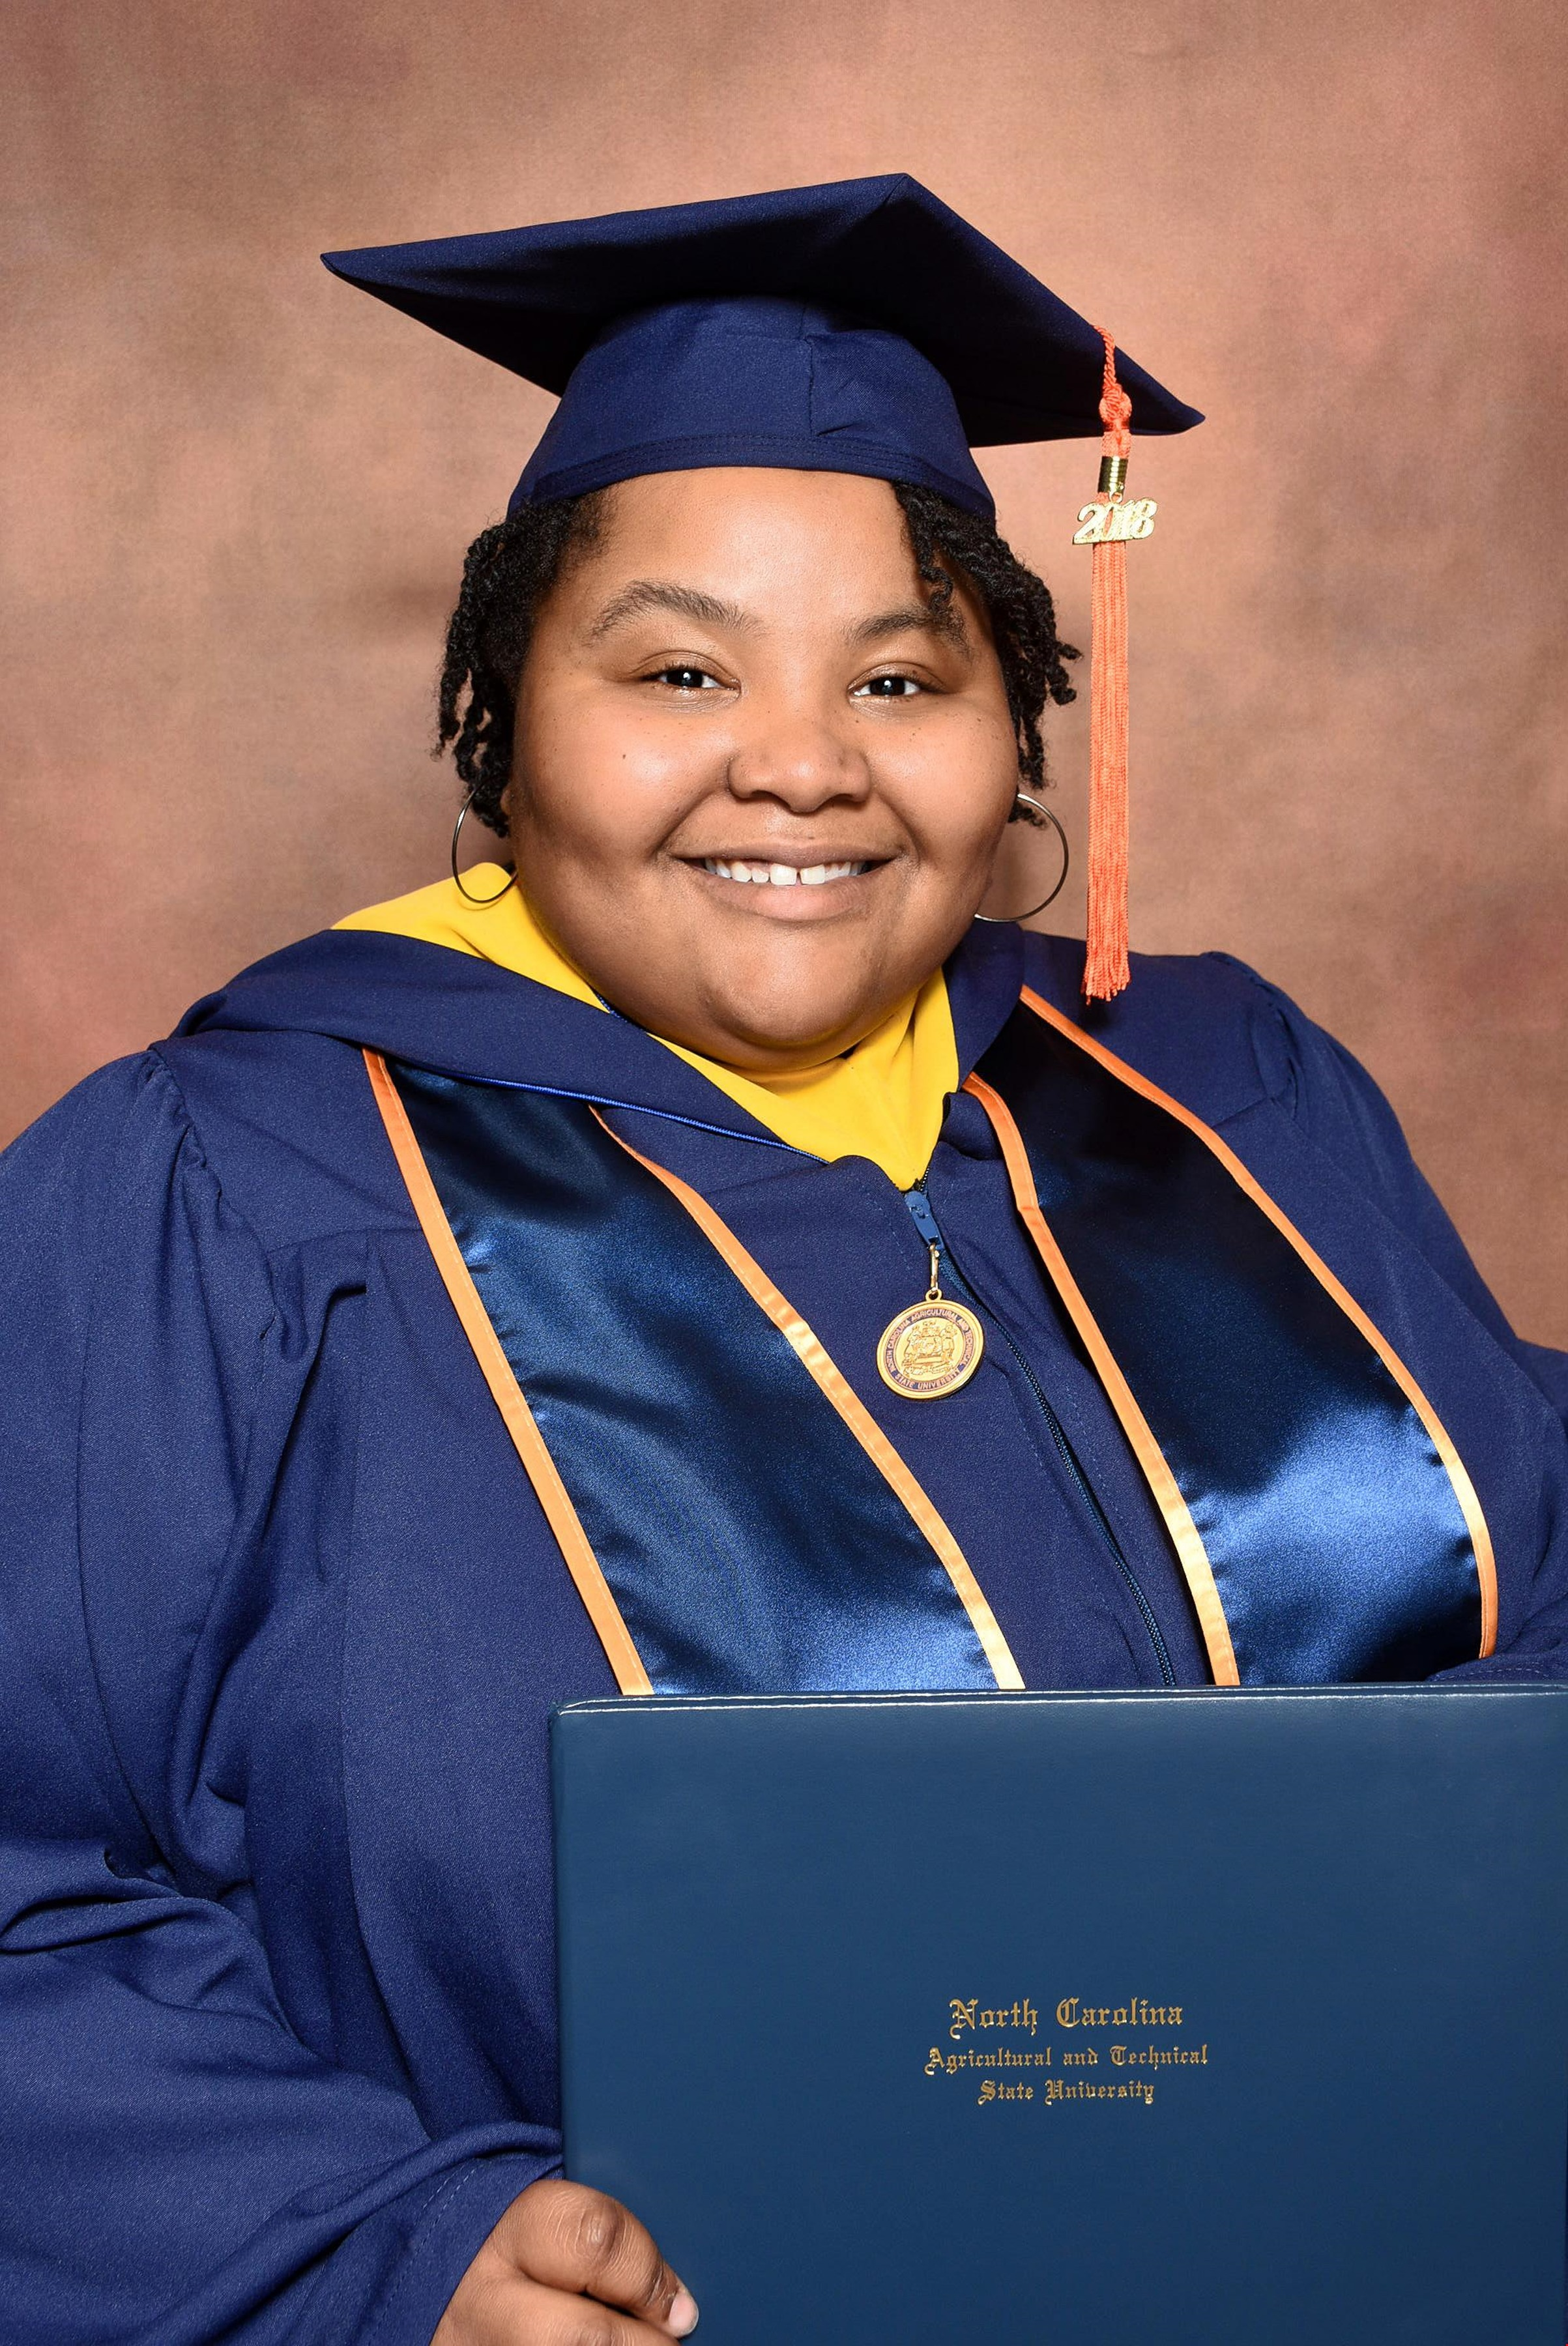
\includegraphics[width= 1in, height= 1.5in]{RosemondGrad.jpg}
    \caption{Photo of the author, Katrina Rosemond.}
\end{figure}

By enrolling in CS 6000, I aim to improve my research skills and 
understand who I am as a researcher. While I have been contributing to 
research projects since undergrad, I still struggle when I lead my 
projects. Mainly when writing, I never knew how much writing was involved 
when I first started in tech. So when I have to write a paper, I struggle 
with determining what's a good paper, pulling out the necessary 
information, and delivering that information on paper. But I know that the 
more I practice, the more I become comfortable with something. Therefore, 
I hope that between the lessons and assignments in CS 6000, I will learn 
to become a better scientific writer and more comfortable when I need to 
write a research paper.

\section{Git Repo}
The synCAN git repo \url{https://github.com/etas/SynCAN} is a synthetic 
controller area network (CAN) dataset used for CAN intrusion detection 
systems (IDSs). I'm currently researching the quality of CAN IDS datasets.

\section{Questions}
\textbf{Question 1:}
\newline
\textbf{Answer 1:}
\newline
\textbf{Question 2:}
\newline
\textbf{Answer 2:}
\newline
\textbf{*FOR THOSE WHO WILL ADD TO THE DOCUMENT PLEASE REMOVE THE 'BEGIN' AND 'END' PREAMBLES OR THE REST OF DOCUMENT WILL NOT SHOW*}
\section{Introduction -- Vijay Banerjee}
I am currently in the 2nd year of PhD program in Computer Science. My research focuses on
security in real-time cyber-physical systems (CPS). I am working on integrating detection,
prevention, and recovery strategies in CPS with real-time guarantees for security and time-
critical applications like flight software. I also like to explore real-time scheduling theory and
implementation challenges in real-time operating systems (RTOS). I genuinely smile when I work on these
ideas, unlike my photo in Fig. 1.
My goal for this course is to understand the general research methodologies used in computer
science (CS) to expand my idea of research and find my paradigm
of research. I am also looking forward to learning the best practices of research and the
common tools that are used across different disciplines to improve efficiency. Through the
class activities and interaction with my peers, I will be able to see different perspectives and
interests, which can open doors to future collaborations and intriguing discussions.
I enjoy playing classical music on the flute in my free time. I also enjoy cooking different
cuisines whenever I find an opportunity
\begin{figure}[h]
    \centering
    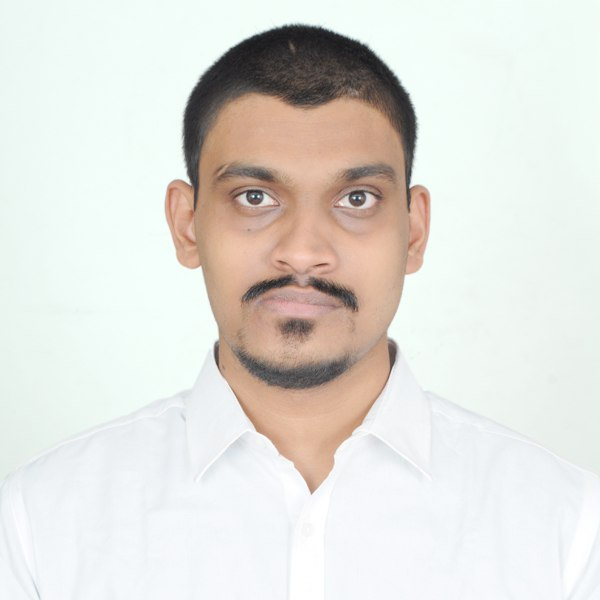
\includegraphics{banerjee.jpeg}
    \caption{This is me (I am not this grumpy in real life)}
    \label{fig:me}
\end{figure}


\section{Related Code Repo}

I am working with Real-Time Operating Systems. One of the most prominent hard RTOS is Real-Time Executive for Multiprocessor Systems (RTEMS). RTEMS has been an open-source organization for over $25$ years, and the code can be found in the following repository:
\url{https://github.com/RTEMS/rtems}



\section{Questions}

\title{Introduction To Research}
\author{Omolade Ikumapayi}
\date{August 2022}

\maketitle

\section{Introduction}

\begin{figure}[h!]
  \centering
  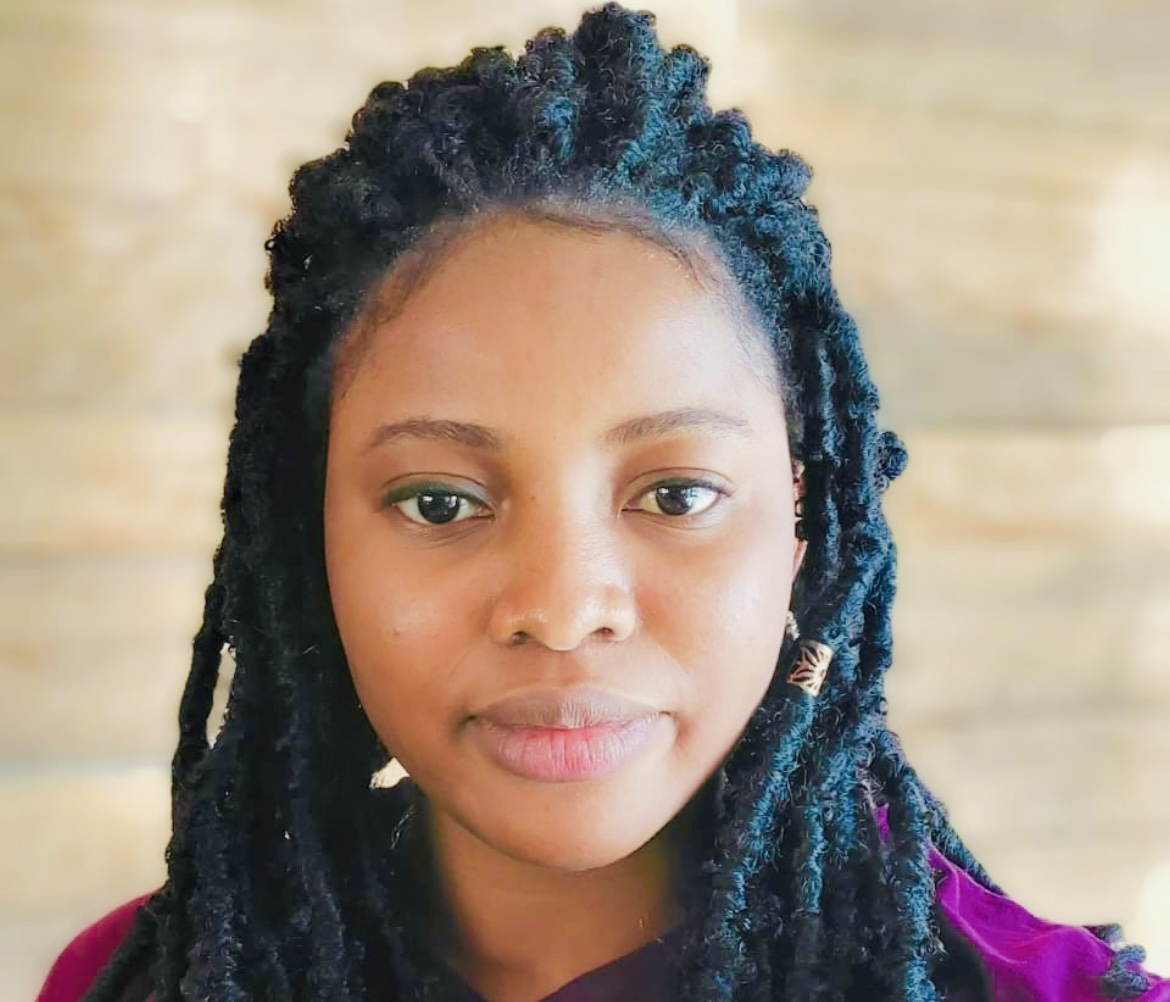
\includegraphics[width=0.5\textwidth]{omolade_.jpg}
\end{figure}

I am a second-year Ph.D. student in the department of computer science at the University of Colorado, Colorado Springs. I work with Dr.Gedare Bloom at the Embedded System Security Laboratory on real-time systems security. Currently I am investigating scheduling algorithms for automotive applications. My goal for taking Introduction to Research class is to get better at research. I believe research is a process and I want to go through the cycle. I consider myself to be creative as I enjoy designing, yet it can be difficult to put ideas into words, and have a thorough statistical and technical representation through the examination of my ideas.
I hope to explore and understand sophisticated scientific publications through this course, which will assist me to get past my research challenges. As someone who wants to increase the caliber of her research, I am also taking this course to network with others who share my interests.
Finally, I believe that by the end of the class, I will have gained the necessary knowledge, skills, and experience to  maximize my potential. With in-depth research, I hope to improve my understanding of the nuances of Cyber-physical systems and take advantage of the opportunity to be taught by the course coordinator. I intend to contribute to the field by applying my theoretical knowledge and scientific ingenuity.
\section{Git Repository}

\url{https://gitlab.com/ipvs/nesting}
\section{Questions}
\subsection{Question 1}

Hi Omolade. Your goal is spot on! Do you intend to do more research or more teaching after the program or maybe a combination of both? Thanks ..Rono
Thanks Rono, I would prefer to do more research to teaching.

\subsection{Question 2}
Have you narrowed down your reserach to any particular cyber-physical system yet? - Dustin Trujillo
Hi Dustin. Yes, right now I am focusing on automotive networks.

\include{rcheruiy}
\documentclass{article}
\usepackage{hyperref, graphics}
\begin{document}
\title{Git Assignment Week 4 }
\maketitle
\section{Introduction:}

I am Minhajul Alam Rahat, a second-year PhD student at the UCCS CS department. My research focus is on embedded system security. Specifically, I am interested in device firmware vulnerability analysis. I am an enthusiast of technology and knowledge. I like practical problem-solving and innovation. I want to contribute to society through my research work in the future. I look forward to working in academia to continue my research work in the future and, at the same time, help students become good researchers.
I look forward to learning research methodologies in a more systematic approach while doing the CS 6000 course. I believe that it will help me broaden my thinking while trying to devise a plan or methodology to solve a problem. This course will also help me read research papers efficiently and hone my skills in using different tools for my research work. I have already met several creative and skilled research people in the class, and I am excited to share our ideas and passions for research. I hope to understand how other people in the research community are doing research in their respective fields. 

\begin{figure}[h]
    \centering
    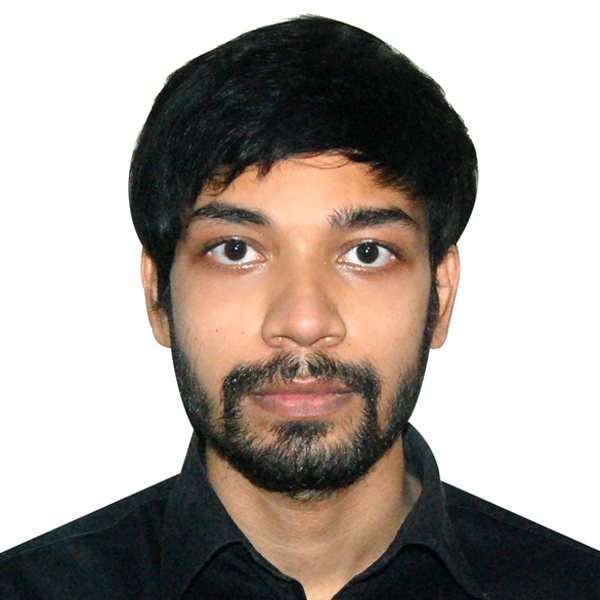
\includegraphics{minhajul.jpg}
    \caption{My Photo ID}
    \label{fig:personalPic}
\end{figure}

\section{Related Code:}

I am working in firmware binary analysis techniques. One of the work related to my topic is Firmalice. Firmalice is a binary firmware analysis framework. It is based on a symbolic execution engine which can find authentication bypass flaws in embedded device firmware. Link to the code for this framwork: 

\url{https://github.com/angr/pyvex}

\section{Questions:}
\end{document}

\documentclass[a4paper]{article}
\usepackage{datetime}
\newdate{date}{20}{09}{2022}
\date{\displaydate{date}}

%% Language and font encodings
\usepackage[english]{babel}
\usepackage[T1]{fontenc}
\usepackage{float}

%% Sets page size and margins
\usepackage[a4paper,top=3cm,bottom=2cm,left=3cm,right=3cm,marginparwidth=1.75cm]{geometry}

%% Useful packages
\usepackage{textcomp}
\usepackage{amssymb}
\usepackage{amsmath}
\usepackage{graphicx}
\usepackage[colorinlistoftodos]{todonotes}
\usepackage[colorlinks=true, allcolors=blue]{hyperref}

\title{Trujillo}
\author{Dustin J. Trujillo}

\begin{document}
\maketitle

%%\begin{abstract}
%%To be added later.
%%\end{abstract}

\section{Introduction}

My name is Dustin Trujillo and I am a second year PhD student in the Security program, advised by Dr. Li. The skills I have gained through my academic studies and 15 years working full-time in the information technology and information security fields have ultimately let me to pursue a PhD in security out of sheer passion for the field and a desire to contribute to it.

I have a diverse working background in project management, military intelligence, cyber threat intelligence, ethical hacking, malware reversal, network security, and designing and implementing secure on-premise and cloud solutions. However, my primary goals for this PhD program and research are to contribute something new and interesting, and of course, useful, to the field of Information and Cybersecurity, specifically in the subset field of Denial of Service (DoS).

While I am still narrowing down (with Dr. Li) my specific dissertation research proposal, I do get excited about topics like network security/threat hunting/ethical hacking/malware reversal. My goal for this class is to completely narrow down my research topic (which is currently Denial of Service) and have my dissertation proposal completed and ready to be presented to the PhD program committee by the end of this 2022 fall semester. 

As far as a few personal items, I love to ski and be outdoors, and my wife and I have 5 kids (blended family) with one on the way! See Figure 1 for a picture of myself.

\begin{figure}[H]
\centering

\includegraphics[width=0.3\textwidth]{trujillo.jpg}
\caption{\label{fig:Me}This is a picture of myself.}
\end{figure}


\section{Data on GitHub}
This \href{https://github.com/vz-risk/VCDB}{VCDB: VERIS Community Database} Git repo has code related to my Denial of Service research area. This repo is the VERIS Community Database and includes a lot of data related to data breaches over the past many years. It is the data source that Verizon uses to test/prove/disapprove their assumptions while developing their annual Data Breach report.

\section{Questions To Answer}

\end{document}

\section{Wes Robbins}
I am in the master's in computer science program at UCCS. My research area is in Computer Vision, Machine Learning, and Biometrics. In particular, I am working on improving biometric robustness in challenging imaging conditions. My goals for this course are to improve my understanding of the process of research and improve my ability to execute high-quality research. 

\section{Repo link}
A repository related to my research is \textit{insightface},
which can be found at\newline \url{https://github.com/deepinsight/insightface}. \\
This repository has code for a number of research problems related face biometrics such as face detection, face alignment, and face recognition. The well maintained over the last several years and includes code for 7 papers that have been published at computer vision conferences.


\begin{figure}[h]
    \centering
    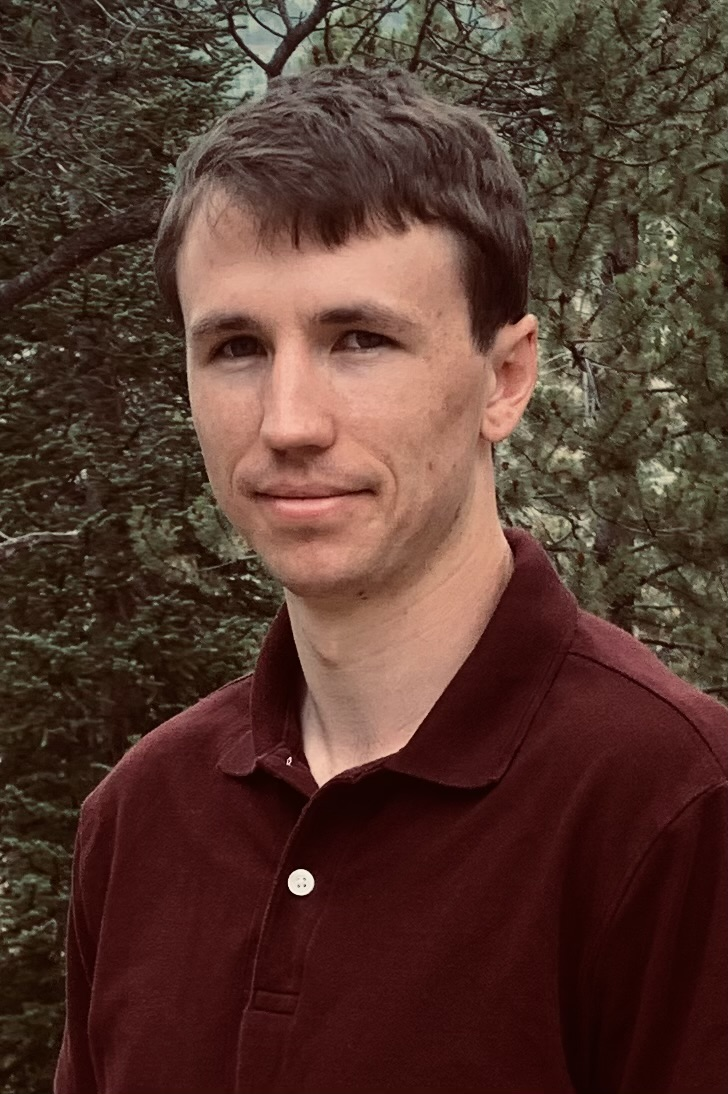
\includegraphics[width=.25\textwidth]{robbins.jpg}
    % \label{fig:my_label}
\end{figure}

\section{Question 01}
What is you plan about boimetrics systems?

% \documentclass[journal]{IEEEtran}

% \usepackage{flushend} % For end of document
% \usepackage{graphicx,color}
% \usepackage[super]{nth}
% \usepackage{wrapfig}
\graphicspath{./images/}
\pagestyle{plain}

% \title{CS6000 \nth{1} Journal}
\author{Mark Maldonado}
\date{August 2022}

% \begin{document}

    \maketitle

    \section{Course Goals}
    \label{sec:Goals}
        \begin{wrapfigure}{L}{0.25\textwidth}
            \centering
            
\includegraphics[width=0.25\textwidth]{images/maldonado_profile.jpg}
        \end{wrapfigure}
        My course goals for this class is to learn better habits to conducting research.
        Since I am already doing research in the cybersecurity domain professionally, I would like to discover new ways to conduct research.
        Doing the bear minimum while reading papers and posting on open-source forums will only take you so far for understanding the field of study.
        The ability to inherit multiple ways to investigate the field of study to achieve your research goals is critical to becoming a sound researcher.

        For my PhD I am researching a novel means to deploy and build honeypots by implementing them with a novel architecture and framework.
        The research behind the honeypots will provide improved methods to deceiving malicious attackers from penetrating production networks and attacking the decoys instead.
        Integrating these deployments and intelligence collection with machine learning algorithms will improve the overall network security stature.
        Machine learning will also be used in log aggregation and decision making for humans to approve or deny of autonomous deployment capabilities.

        I intend to build a company out of this research and hope to help improve the global security of enterprise networks.
        This is one of my main goals after completing my PhD amongst other side projects I still intend to complete.
        As a hobby I do a ton of side programming for my family creating multiple gadgets using either arduino or a raspberry pi's.
        Each of my siblings have gotten a small gadget they requested to help with every-day life in their household.

    \section{Related Code Base}
    \label{sec:code}
        I found an open source ecosystem for deploying honeypots using a LAMP stack.
        This software is managed by a group of people and has a decent amount of support for it.
        The software is capable of monitoring and manage the deployed honeypots.
        Their git repository is named \href{https://github.com/honeytrap/honeytrap}{Honeytrap}.

    \section{Ask Questions}

    \textbf{Q1:} Hi Mark. Your research topic is quite interesting! Can you elaborate on how the deployed architecture with honeypots is combined with machine learning to improve network security? Thanks.
    \newline
    The architecture is cloud based and is capable if being deployed to multiple cloud providers. This is deliberate since cloud computing is what most networks are comprised of. The architecture is just the inner workings of how everything is deployed. The framework will have multiple servers capable of gathering logs to shape and label data for a machine learning engine. There are multiple aspects I do not wish to discuss about the machine learning portions since it'll be patent able or proprietary to the company I'll be starting. To keep it short it'll be apart of the back-bone of how to deploy honeypots in a production network space.


    % \flushend

% \end{document}

\documentclass[11pt, letterpaper]{article}
\usepackage[margin=1in,letterpaper]{geometry}
\usepackage{graphicx,float}
\usepackage{hyperref}
\hypersetup{colorlinks = true, urlcolor=blue, filecolor=blue, citecolor = black,linkcolor=black}

\begin{document}
\section{Personal biography}
I, H. M. A. Mohit Chowdhury, started Ph.D. in Computer Science at the University of Colorado at Colorado Springs in Fall 2022. My primary research advisor is Dr. Oluwadare. I will start working as a Graduate Research Assistant with Dr. Boult. I completed my B.Sc. in Computer Science and Engineering in 2017 from Ahsanullah University of Science and Technology, Dhaka. After that, I worked for 5 years as a Software Engineer in national \& multinational companies. At a certain time, I realized that I can contribute by doing research and took decision to pursue Ph.D. degree as a first step. I love site seeing, cooking, bike riding, and gossiping with my friends. My friends call me \textbf{Shadhin} which means \textit{Independent}.

\begin{figure}[H] \center
    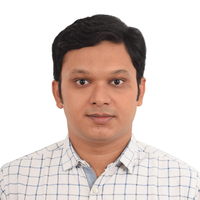
\includegraphics[scale=1]{chowdhury.jpg}
    \caption{H. M. A. Mohit Chowdhury}
    \label{fig:chowdhury}
\end{figure}

\section{One Pixel Attack Git Repository}
Adversarial attack is one of the main concerns in computer vision based algorithms which could demolish a whole system. There are lots of adversarial attacks and one of them is one-pixel attack means changing a single data will cause an unusual result. Here, we can find \href{https://github.com/Hyperparticle/one-pixel-attack-keras}{One Pixel Attack} code for experiencing vulnerability.

\section{Question \& Answer}
\subsection{Question 01} How can an adverserial attack like one pixel attack demolish a whole system? Is it kind of a malware? 
\subsection{Answer 01}
Good question! If you have an image of an square shape and  you are expecting your system should detect it as a square. Suppose, this image edge pixels changed(may be through the network or with some malware) and now  your system will not consider it as a square rather it may say hexagone or any other ususual shape.
\subsection{Question 02}
\subsection{Answer 02}
\section{GIT process}
Here, I forked the repository and created my own branch. After that, I created a pull request to the main repository. Then I checked out one of my peer branch and asked a question and created a pull request to his branch. When I asked second question, and pushed to the main branch, there was a conflict and an unsuccessful push. I pulled the main branch without any conflict and agaign pushed to the main branch.
\end{document}


\section{Fall 2023 Student Content}
\hypersetup{colorlinks=true, urlcolor=blue, linkcolor=black}

% My macros
\newcommand{\myfullname}{Carlos Eugenio Lopes Pires Xavier Torres}
\newcommand{\myshortname}{Carlos E. Torres}

% Title
\title{CS 6000 - Week 5 - Git Assignment}
\author{\myfullname}
\date{\today}

\maketitle

\section{About me}

I am pursuing my PhD in Computer Science since Fall 2021 at the University of Colorado, Colorado Springs. I have worked with Dr. Xu in one of his research projects related to cybersecurity, secure and privacy-preserving data sharing. I created a system on that research that I will present in November at the ISTSS annual meeting in Los Angeles, CA.
I am currently involved in a research project with my new advisor, Dr. Oluwadare, in the Bioinformatics field, researching 3D chromosome and genome structure modeling and visualization.

\begin{wrapfigure}[11]{r}{0.25\textwidth}
    \centering
    
\includegraphics[width=0.25\textwidth]{Torres-F23-photo.jpg}
    \caption{\small My photo}
\end{wrapfigure}

I am currently working full-time as a Principal Software Engineer at Oracle. I work with data science, big data, and full stack web development. My past experience includes working as a senior software engineer, expert in mobile and web solutions development with 22 years experience. Experienced in fast-paced environments, team leadership, client-facing and customer relationship. Also experienced in the whole software development process, from concept, requirements, analysis, database modeling, programming, testing, until production and maintenance.

There are a few ways to contact me and get to know more about my experience, projects, and career. Just visit these links:
\begin{itemize}
    \item LinkedIn: \url{https://linkedin.com/in/cetorres}
    \item GitHub: \url{https://github.com/cetorres}
    \item Twitter: \url{https://twitter.com/cetorres}
    \item Website: \url{https://cetorres.com}
\end{itemize}

\section{A Git repository related to my research}

HiC-GNN is a generalizable model for 3D chromosome reconstruction using graph convolutional neural networks. This work was done in my current research lab (Oluwadare Lab) by Van Hovenga and Oluwatosin Oluwadare. The repository (\url{https://github.com/OluwadareLab/HiC-GNN}) has the code referenced in their paper that is used to train the model and generate the .pdb file containing the predicted 3D structure corresponding to the input file. The input file must be a Hi-C contact map in either matrix format or coordinate list format.

% ---------------------------------
% INSTRUCTIONS FOR QUESTIONS
% Please make your questions below.
% Replace [Question 1] and [Question 2] with your actual questions.
% One question per person.
% ---------------------------------

\section{Questions}

\subsection{[Question 1]}

\subsection{[Question 2]}


Zainab: How are you finding the transition from security-related research to Bioinformatic? 

% \end{document}



\section{Example of Easy Tables}
\csvautotabular{test.csv}


\section*{Better formated Tables}
    \begin{tabular}{r|r|r}%
    % specify table head
    \bf Time (s) & \bf Rel. time (s)& \bf Y Pos
% use head of csv as column names
    \csvreader{test.csv}{}
% specify selected coloumns here
    {\\\hline\csvcoli&\csvcolii&\csvcolvi}
    \end{tabular}
    \clearpage


\end{document}
